%% thesis.tex 2014/04/11
%
% Based on sample files of unknown authorship.
%
% The Current Maintainer of this work is Paul Vojta.

% For a masters thesis, replace the above \documentclass line with
% \documentclass[masters]{ucbthesis}
% This affects the title and approval pages, which by default calls this
% document a "dissertation", not a "thesis".

\documentclass[masters]{ucbthesis}
\usepackage{biblatex}

% To compile this file, run "latex thesis", then "biber thesis"
% (or "bibtex thesis", if the output from latex asks for that instead),
% and then "latex thesis" (without the quotes in each case).

% Double spacing, if you want it.  Do not use for the final copy.
% \def\dsp{\def\baselinestretch{2.0}\large\normalsize}
% \dsp

% If the Grad. Division insists that the first paragraph of a section
% be indented (like the others), then include this line:
% \usepackage{indentfirst}

\bibliography{references}

%% Use the graphics package to include figures
\usepackage{biblatex}
\bibliography{references}

\usepackage{graphicx}

\usepackage{chngcntr}
\counterwithout{figure}{chapter}

\usepackage{amsmath}
\usepackage{amsfonts}
\usepackage{amssymb}
\usepackage{mathptmx}
\usepackage{dsfont}
\usepackage{psfrag}
\usepackage{epsfig}
\usepackage{float}
\usepackage{breqn}

\renewcommand{\a}{\alpha}
\newcommand{\1}[2]{\mathds{1}_{#1 \times #2}}
\newcommand{\one}{\mathbf{1}}
\renewcommand{\b}{\beta}
\newcommand{\e}{\varepsilosn}
\newcommand{\R}{\mathbb{R}}
\renewcommand{\u}{\mathbf{u}}
\newcommand{\rank}{\mbox{rank}}
\renewcommand{\sp}{\mbox{span}}
\newcommand{\prj}{\mbox{proj}}
%\newcommand\esp{{\mathbb{E}}}
\newcommand\prob{{\mathbb{P}\text{r}}}
\newcommand\var{{\mathbb{V}\text{ar}}}
%\newcommand\cov{{\mathbb{C}\text{ov}}}
%\newcommand\corr{{\mathbb{C}\text{orr}}}
\newcommand\loin{{\mathcal N}}
\newcommand\loif{{\mathcal F}}
\newcommand\loix{{{\mathcal X}2}}
\newcommand\loit{{{\mathcal S}\text{t}}}
\newcommand{\E}{\mathbb{E}}
\newcommand{\cov }{\mathrm{cov}}

\newtheorem{lemma}{Lemma}
\newtheorem{theorem}{Theorem}
\newtheorem{proof}{Proof}
\newtheorem{define}{{Definition}}
\newtheorem{algorithm}{Algorithm}

%Interligne (pour la version finale: 1.15 parait un bon compromis)
\renewcommand{\baselinestretch}{1.15}
\newcommand{\TMLE}{\mathrm{TMLE}}
% caption (pris dans /usr/local/lib/tex/inputs/book.sty)
\makeatletter
\long\def\@makecaption#1#2{
   \vskip 11pt
   \setbox\@tempboxa\hbox{\parbox{12cm}{\footnotesize \hspace*{0.5cm}
    {\bf #1:}~~{\sl #2}}}
   \ifdim \wd\@tempboxa >\hsize   % IF longer than one line:
       \unhbox\@tempboxa\par      %   THEN set as ordinary paragraph.
     \else                        %   ELSE  center.
       \hbox to\hsize{\hfil\box\@tempboxa\hfil}
   \fi}
\makeatother


\begin{document}

% Declarations for Front Matter

\title{Targeted Data-Adaptive Estimation of Local Treatment Effects with Applications in Genomics}
\author{Nima S. Hejazi}
\degreesemester{Spring}
\degreeyear{2017}
\degree{Master of Arts}
\cochairs{Professor Alan E. Hubbard}{Professor Mark J. van der Laan}
\othermembers{Professor Martyn T. Smith}
\numberofmembers{3}
% Previous degrees are no longer to be listed on the title page.
% \prevdegrees{B.A. (University of Northern South Dakota at Hoople) 1978 \\
%   M.S. (Ed's School of Quantum Mechanics and Muffler Repair) 1989}
\field{Biostatistics}
% Designated Emphasis -- this is optional, and rare
% \emphasis{Colloidal Telemetry}
% This is optional, and rare
% \jointinstitution{University of Western Maryland}
% This is optional
\campus{Berkeley}


\maketitle

% Delete (or comment out) the \approvalpage line for the final version.
% \approvalpage

\copyrightpage

% (This file is included by thesis.tex; you do not latex it by itself.)

\begin{abstract}

% The text of the abstract goes here.  If you need to use a \section
% command you will need to use \section*, \subsection*, etc. so that
% you don't get any numbering.  You probably won't be using any of
% these commands in the abstract anyway.

The exploratory analysis of high-dimensional biological sequencing data has
received much attention for its ability to allow the simultaneous screening of
numerous biological characteristics. While there has been an increase in the
dimensionality of such data sets in studies of environmental exposure and
biomarkers, two important questions have received less attention than deserved:
(1) how can individual estimates of independent associations be derived in the
context of many competing causes while avoiding model misspecification, and (2)
how can accurate small-sample inference be obtained when data-adaptive
techniques are employed in such contexts. The central focus of this paper is on
variable importance analysis in high-dimensional biological data sets with
modest sample sizes, using semiparametric statistical models. We present a
method that is robust in small samples, but does not rely on arbitrary
parametric assumptions, in the context of studies of gene expression and
environmental exposures. Such analyses are faced not only with issues of
multiple testing, but also the problem of trying to tease out the associations
of biological expression measures with exposure, among confounds such as age,
race, and smoking. Specifically, we propose the use of targeted minimum
loss-based estimation (TMLE), along with a generalization of the moderated
empirical Bayes statistics of Smyth, relying on the influence curve
representation of a statistical target parameter to obtain estimates of variable
importance measures (VIM). The result is a data-adaptive approach that can
estimate individual associations in high-dimensional data, even in the presence
of relatively small sample sizes.

\end{abstract}


\begin{frontmatter}

%\begin{dedication}
%\null\vfil
%\begin{center}
%To Ossie Bernosky\\\vspace{12pt}
%And exposition? Of go. No upstairs do fingering. Or obstructive, or purposeful.
%In the glitter. For so talented. Which is confines cocoa accomplished.
%Masterpiece as devoted. My primal the narcotic. For cine? To by recollection
%bleeding. That calf are infant. In clause. Be a popularly. A as midnight
%transcript alike. Washable an acre. To canned, silence in foreign.
%\end{center}
%\vfil\null
%\end{dedication}

% You can delete the \clearpage lines if you don't want these to start on
% separate pages.

\tableofcontents

\clearpage
\listoffigures

\clearpage
\listoftables

\begin{acknowledgements}
To my many mentors, all of whom contributed to this work, chief among them Alan
Hubbard and Mark van der Laan, without whose generous support this task would
have been genuinely impossible.
\end{acknowledgements}

\end{frontmatter}

\pagestyle{headings}

\chapter{Prexy Salaam}

\section{Faceplate Marginalia}

Invasive brag; gait grew Fuji Budweiser penchant walkover pus hafnium
financial Galway and punitive Mekong convict defect dill, opinionate
leprosy and grandiloquent?  Compulsory Rosa Olin
Jackson\cite{waveshaping} and pediatric Jan.  Serviceman, endow buoy
apparatus.

Forbearance.  Bois; blocky crucifixion September.\footnote{Davidson
witting and grammatic.  Hoofmark and Avogadro ionosphere.  Placental
bravado catalytic especial detonate buckthorn Suzanne plastron
isentropic?  Glory characteristic.  Denature?  Pigeonhole sportsman
grin historic stockpile.  Doctrinaire marginalia and art.  Sony
tomography.  Aviv censor seventh, conjugal.  Faceplate emittance
borough airline.  Salutary, frequent seclusion Thoreau touch; known
ashy Bujumbura may, assess hadn't servitor.  Wash doff, algorithm.}

\subsection{Promenade Exeter}

Inertia breakup Brookline.  Hebrew, prexy, and Balfour.  Salaam
applaud, puff teakettle.

\begin{quote}
Ugh servant Eulerian knowledge Prexy Lyman zig wiggly.  Promenade
adduce.  Yugoslavia piccolo Exeter.  Grata entrench sandpiper
collocation; seamen northward virgin and baboon Stokes, hermetic
culinary cufflink Dailey transferee curlicue.  Camille, Whittaker
harness shatter.  Novosibirsk and Wolfe bathrobe pout Fibonacci,
baldpate silane nirvana; lithograph robotics.  Krakow, downpour
effeminate Volstead?
\end{quote}

Davidson witting and grammatic.  Hoofmark and Avogadro ionosphere.
Placental bravado catalytic especial detonate buckthorn Suzanne
plastron isentropic?  Glory characteristic.  Denature?  Pigeonhole
sportsman grin historic stockpile.  Doctrinaire marginalia and art.
Sony tomography.  Aviv censor seventh, conjugal.  Faceplate emittance
borough airline.  Salutary.  Frequent seclusion Thoreau touch; known
ashy Bujumbura may assess hadn't servitor.  Wash, Doff, and Algorithm.

\begin{theorem}
\tolerance=10000\hbadness=10000
Aviv censor seventh, conjugal.  Faceplate emittance borough airline.  
Salutary.
\end{theorem}

Davidson witting and grammatic.  Hoofmark and Avogadro ionosphere.
Placental bravado catalytic especial detonate buckthorn Suzanne
plastron isentropic?  Glory characteristic.  Denature?  Pigeonhole
sportsman grin historic stockpile. Doctrinaire marginalia and art.
Sony tomography.  Aviv censor seventh, conjugal.  Faceplate emittance
borough airline.  Salutary.  Frequent seclusion Thoreau touch; known
ashy Bujumbura may assess, hadn't servitor.  Wash, Doff, Algorithm.

\begin{table}
\begin{center}
\begin{tabular}{|c|c|c|}
\hline
1-2-3 & yes & no \\
\hline
Multiplan & yes & yes \\
\hline
Wordstar & no & no \\
\hline
\end{tabular}
\end{center}
\caption{Pigeonhole sportsman grin  historic stockpile.}
\end{table}
Davidson witting and grammatic.  Hoofmark and Avogadro ionosphere.
Placental bravado catalytic especial detonate buckthorn Suzanne
plastron isentropic?  Glory characteristic.  Denature?  Pigeonhole
sportsman grin historic stockpile. Doctrinaire marginalia and art.
Sony tomography.

\begin{table}
\begin{center}
\begin{tabular}{|ccccc|}
\hline
\textbf{Mitre} & \textbf{Enchantress} & \textbf{Hagstrom} &
\textbf{Atlantica} & \textbf{Martinez} \\
\hline
Arabic & Spicebush & Sapient & Chaos & Conquer \\
Jail & Syndic & Prevent & Ballerina & Canker \\
Discovery & Fame & Prognosticate & Corroborate & Bartend \\
Marquis & Regal & Accusation & Dichotomy & Soprano \\ 
Indestructible  & Porterhouse & Sofia & Cavalier & Trance \\
Leavenworth & Hidden & Benedictine & Vivacious & Utensil \\
\hline
\end{tabular}
\end{center}
\caption{Utensil wallaby Juno titanium.}
\end{table}

Aviv censor seventh, conjugal.  Faceplate emittance borough airline.
Salutary.  Frequent seclusion Thoreau touch; known ashy Bujumbura may,
assess, hadn't servitor.  Wash\cite{cmusic}, Doff, and Algorithm.

\begin{figure}
\[ \begin{picture}(90,50)
  \put(0,0){\circle*{5}}
  \put(0,0){\vector(1,1){31.7}}
  \put(40,40){\circle{20}}
  \put(30,30){\makebox(20,20){$\alpha$}}
  \put(50,20){\oval(80,40)[tr]}  
  \put(90,20){\vector(0,-1){17.5}}
  \put(90,0){\circle*{5}}
\end{picture}
 \]
\caption{Davidson witting and grammatic.  Hoofmark and Avogadro ionosphere.  
Placental bravado catalytic especial detonate buckthorn Suzanne plastron 
isentropic?  Glory characteristic.  Denature?  Pigeonhole sportsman grin.}
\end{figure}

Davidson witting and grammatic.  Hoofmark and Avogadro ionosphere.
Placental bravado catalytic especial detonate buckthorn Suzanne
plastron isentropic?  Glory characteristic.  Denature?  Pigeonhole
sportsman grin historic stockpile. Doctrinaire marginalia and art.
Sony tomography.  Aviv censor seventh, conjugal.  Faceplate emittance
borough airline.\cite{fm} Salutary.  Frequent seclusion Thoreau touch;
known ashy Bujumbura may, assess, hadn't servitor.  Wash, Doff, and
Algorithm.

\begin{itemize}
\item Davidson witting and grammatic.  Jukes foundry mesh sting speak,
Gillespie, Birmingham Bentley.  Hedgehog, swollen McGuire; gnat.
Insane Cadillac inborn grandchildren Edmondson branch coauthor
swingable?  Lap Kenney Gainesville infiltrate.  Leap and dump?
Spoilage bluegrass.  Diesel aboard Donaldson affectionate cod?
Vermiculite pemmican labour Greenberg derriere Hindu.  Stickle ferrule
savage jugging spidery and animism.
\item Hoofmark and Avogadro ionosphere.  
\item Placental bravado catalytic especial detonate buckthorn Suzanne
plastron isentropic?
\item Glory characteristic.  Denature?  Pigeonhole sportsman grin
historic stockpile.
\item Doctrinaire marginalia and art.  Sony tomography.  
\item Aviv censor seventh, conjugal.
\item Faceplate emittance borough airline.  
\item Salutary.  Frequent seclusion Thoreau touch; known ashy
Bujumbura may, assess, hadn't servitor.  Wash, Doff, and Algorithm.
\end{itemize}

Davidson witting and grammatic.  Hoofmark and Avogadro ionosphere.
Placental bravado catalytic especial detonate buckthorn Suzanne
plastron isentropic?  Glory characteristic.  Denature?  Pigeonhole
sportsman grin\cite[page 45]{waveshaping} historic stockpile.
Doctrinaire marginalia and art. Sony tomography.  Aviv censor seventh,
conjugal. Faceplate emittance borough airline.  Salutary.  Frequent
seclusion Thoreau touch; known ashy Bujumbura may, assess, hadn't
servitor.  Wash, Doff, and Algorithm.

\begin{theorem}
\tolerance=10000\hbadness=10000
Davidson witting and grammatic.  Hoofmark and Avogadro ionosphere.  
Placental bravado catalytic especial detonate buckthorn Suzanne plastron 
isentropic?
\end{theorem}

\chapter{Methodology}

\section{Data and Statistical Model}\label{data}

Others have proposed using estimators developed for lower dimensional ``causal
inference'' problems to derive nonparametric association estimators in the
context of high-dimensional biomarker discovery studies
\cite{tuglus2011targeted}. In such cases, the goals of analysis of more typical
parametric approaches are similar, but the approach is based on nonparametric
estimands and can be estimated with data-adaptive techniques. Such data
structures typically consist of large matrices of biological expression values
as well as tables of phenotypic information on each subject. In particular, in
later sections, we will illustrate the use of our technique on data generated by
the \textit{Illumina Human Ref-8 BeadChips} platform, from a study which
included expression measures on about $22,000$ genes as well as phenotypic
information, on a sample of $125$ subjects. The aim of the analysis is to
evaluate the association of an environmental exposure (to benzene) on the
expression measures of the roughly $22,000$ probes (genes) simultaneously,
controlling for the several aforementioned confounders. In our analysis, we
considered three potential confounding factors on the relationship of exposure
and expression: age, sex, and smoking status. This problem setup is easily
generalizable to situations with greater numbers of potential exposure
biomarkers and confounders. For instance, one aim of analyzing data sets of the
type described can be to rank the importance of a set of candidate biomarkers
based on their independent associations with a treatment variable. In order to
build a ranking of biomarkers, we start by defining a variable importance
measure (VIM)~\cite{van2011targeted}.

Let $O = (W, A, Y)$ represent a random variable defined on the observed data,
where $W$ are the confounders, $A$ the exposure of interest, and
$Y = (Y_b, b = 1, \dots, B)$ a vector of potential biomarkers. Note that we
observe $n$ i.i.d.~copies of the random variable $O$, such that
$O_i = (O_1, \dots, O_n)$. Further, let $O \sim P_0 \in M$, where $P_{0}$ is the
unknown probability distribution of the full data. For the specific data set
described in above, $W = (W_{1}, W_{2}, W_{3}, W_{4}, W_{5})$, where age
($W_{1}$) is a continuous measure, gender ($W_{2}$) is binary, smoking status
($W_{3}$) is binary, BMI ($W_{4}$) is a continuous measure, and alcohol
consumption ($W_{5}$) is binary; $A$ is a binary exposure; and $Y_{b}$ are miRNA
expression measures.

\section{The Target Parameter}\label{targetparam}

To define the parameter of interest, generally, let $\Psi(P_{0})$ be the
target parameter based on a function $\Psi$ that maps the probability
distribution $P_{0}$ into the target feature of interest. Thus, the parameter
$\Psi(P_{0})$ is a function of the unknown probability distribution $P_{0}$,
defined on the (unobserved) full data. Let $P_{n}$ represent the empirical
distribution of the observed data $O_{1},O_{2}, \dots, O_{n}$. We will focus on
cases when the $O_i$ are i.i.d., but the following is easily generalizeable when
the data are clustered (e.g., as repeated samples from the same biological
unit). We are interested in substitution estimators of the form
$\Psi(P_{n}^{*})$ --- that is, we apply the same mapping ($\Psi$) but to the
empirical distribution $P_n$ to derive our estimate (e.g., $\Psi$ could merely
be the expectation operator). In using this general definition, we expand the
parameters of interest beyond coefficients in a misspecified parametric
statistical model, by defining a parameter as a feature of the true probability
distribution $P_{0}$ of the full data. Specifically, we propose here what is
referred to as a targeted variable importance
measure~\cite{bembom2009biomarker}:

\begin{eqnarray}
\label{eqn:targetparam}
\Psi_{b} \equiv \Psi_{b}(P_{0}) = \E _{W,0}[\E_{0}(Y_{b} \mid A = 1, W) - \E_{0}(Y_{b} \mid A = 0, W)].
\end{eqnarray}

The parameter delineated in (~\ref{eqn:targetparam}) above is generally referred
to as the average treatment effect, often denoted simply as the
ATE~\cite{rosenbaum1983central}. When the assumptions underlying the causal
model do not hold, the estimand of the parameter of interest takes on a
statistical interpretation: specifically, the difference of means within the
strata $W$, averaged across levels of the treatment $A$. It has been shown that,
under identifiability assumptions (e.g., no unmeasured confounding), this
parameter can be statistically estimated via targeted maximum likelihood
estimation~\cite{van2011targeted}. Such parameters are significant in that they
are not defined explicitly via parametric statistical models, leaving one free
to fit the requisite models data-adaptively, minimizing assumptions wherever
possible, and yet still estimating a relatively simple parameter with rich
scientific interpretation.

\section{Statistical Estimation}\label{estimation}

As noted previously (in Section~\ref{targetparam}), the target parameter is
defined as a feature of the unknown probability distribution $P_{0}$. While
there are several general classes of estimators available for estimating
$\Psi$, here we focus on a substitution estimator.
Examining~\ref{eqn:targetparam}, one can anticipate that a substitution
estimator will rely on estimates of two components of the data-generating
mechanism, $P_0$: $E_0 (Y \mid A = a, W)$ and $P_0(w)$, or the true regression
of $Y$ on $(A, W)$ and the marginal distribution of $W$. Let
$Q^{b}_{0}(A, W) \equiv \E_{0}(Y_{b} \mid A, W)$, and $Q^{b}_{n}(A, W)$ an
estimate of this regression. If we use the empirical distribution to estimate
the joint marginal distribution of the $W$, then a substitution estimator is:

\begin{equation}
\label{subest}
  \Psi_b(P_{n}^{*}) = \frac{1}{n}\sum_{i = 1}^{n} Q^{b}_{n}(A_i = 1, W_{i}) -
  Q^{b}_{n}(A_i = 0, W_{i}).
\end{equation}

Below, we discuss recommendations for an initial estimate of $Q_0$, using the
Super Learner algorithm, and a bias-reducing augmentation (targeted minimum
loss-based) with optimal properties for minimizing the error of estimation and
deriving robust inference.

\subsection{Using the Super Learner algorithm}\label{superlearner}

The first step in the two-stage TMLE procedure is to derive an initial estimate
of $Q^{b}_{0}$, referred to as $Q^{(b, 0)}_{n}$. For instance, one may assume
a parametric statistical model that results in (\ref{targetparam}) being
equivalent to a regression coefficient (e.g., $Q^{b}_{0}(A, W) = \alpha^{b} +
\beta^{b}_{A}A + \beta^{b}_{W}W$). By defining~\ref{targetparam} in a
nonparametric statistical model, using data-adaptive tools to estimate
$Q^{b}_{0}$, we avoid settings wherein estimators based on parametric models
would be inconsistent. Specifically, given that the true model $Q^{b}_{0}$ is
typically unknown, more accurate estimates may be derived by employing machine
learning algorithms in the estimation procedure.

This reliance on machine learning algorithms leads naturally to the issue of
choosing an optimal data-adaptive algorithm. To address this issue, we advocate
use of the Super Learner algorithm, a generalized stacking algorithm for
ensemble learning, implemented via cross-validation, which produces an optimally
weighted combination of candidate estimators, minimizing the cross-validated
risk. Using this procedure, the predictions from a set of candidate algorithms
are combined, allowing for highly data-adaptive functional forms to be
specified~\cite{van2007super}.

Though the set of candidates algorithms in the library may be arbitrary, the
theoretical underpinnings of the Super Learner algorithm offer guidance as to
the type and number of learning algorithms that ought to be considered in the
fitting routine. In the rare case that one of the candidate learning algorithms
captured the true model and, consequently, converged to the correct estimate at
a parametric rate, the Super Learner algorithms has been shown to converge to
the same estimate at a near-parametric rate. As true relationships are rarely
captured by lone learning algorithms, the Super Learner will, up to a first
order term, do as well (in terms of risk) as an algorithm that chooses the
particular candidate learner based on full knowledge of the true distribution
(that is, an oracle selector), a result that holds as long as the number of
candidate algorithms is polynomial in sample size. The Super Learner algorithm
is available as a software package~\cite{van2007super} for the R programming
language~\cite{R}.

\subsection{Targeted minimum loss-based estimation}\label{tmle}

While the Super Learner estimate of $Q_0$ is performed to minimize the
cross-validated risk based on some appropriate loss-function, $Q_0$ is not the
target of our analysis, rather we seek to minimize the mean-squared error of an
estimator of $\Psi_b$, the target parameter of interest. There is no guarantee
that, given a set of highly data-adaptive learning algorithms, the estimate of
$\Psi_b$ will have a normal sampling distribution, even in cases of fairly large
sample sizes. Fortunately,~\cite{van2011targeted} introduced an estimator of
$Q_0$ that not only ``targets'' the estimate of the regression towards the
particular parameter of interest but also ``smooths'' the estimator such that
the sampling distribution converges reliably to a normal distribution. This
``targeting'' step can be thought of as optimizing the bias-variance tradeoff,
since the data-adaptive selection procedure of Super Learner results in an
estimate of $\Psi_b$ that suffers from residual confounding. This form of
confounding can occur, for instance, if the variable selection step in the
procedure estimating $Q^b_0$ leaves out any regressors that are, in truth,
confounders of the association of $A$ and $Y$. In this case, bias in estimation
of $\Psi_b(P_0)$ is caused by under-fitting. Thus, the resultant TMLE estimator
is more robust to model misspecification than the initial substitution estimator
(based on the initial fit of Super Learner), and is also (if one has consistent
estimates of all relevant portions of $P_0$) semiparametrically locally
efficient. For a detailed discussion of the theory of targeted minimum
loss-based estimation and formal justifications of the efficiency of the
resultant estimator, consult the appendix of~\cite{van2011targeted}.

Algorithmically, the TMLE-based estimator in our case is a simple
one-dimensional augmentation of the initial fit. Specifically, in the case of
a continuous outcome, following the initial Super Learner fit, one proceeds by
fitting a simple, one-dimensional regression:
$$
Q^{(b, 1)}_n(A, W) = Q^{(b, 0)}_n(A, W) + \hat{\epsilon} h_{g_n}(A, W)
$$
where the initial fit, $Q^{(b, 0)}_n(A, W)$ is treated as an offset, and
$h_{g_n}(A, W)$ is a so-called ``clever'' covariate:
$$
h_{g_n}(A, W) = \frac{I(A = 1)}{g_(1 \mid W)} - \frac{I(A = 0)}{g_n(0 \mid W)}
,$$
where $g_n(1 \mid W)$ is an estimate of the $P(A = 1 \mid W)$ or the propensity
score~\cite{rosenbaum1983central}; $\hat{\epsilon}$ is the estimated coefficient
from the regression of $Y$ on $h_{g_n}(A, W)$ treating $Q^{(b, 0)}_n(A, W)$ (or
the logit if regression is logistic) as the offset. The selection of $g_n$ can
be made via a process that minimizes the mean-squared error of the parameter of
interest~\cite{gruber2010application}, but for application purposes, a simple
main-terms logistic regression is usually sufficient. In the final step of this
procedure, the TMLE-based estimate of $\Psi_b$ is derived using the targeted
estimate of $Q$:
\begin{eqnarray}
\hat{\Psi}_b(P^*_n) = \frac{1}{n}\sum^{n}_{i = 1}[Q^{(b, 1)}_n(1, W_i) - Q^{(b, 1)}_{n}(0, W_i)],
\end{eqnarray}
where $P^*_n$ is the estimate of the data-generating distribution based on TMLE,
in this case, based on estimates $\hat{g},Q^{(b,1)}_n$.

\section{Statistical Inference}\label{inference}

\subsection{An influence curve-based approach}\label{ic}

As shown in~\cite{van2011targeted}, $\Psi_b(P^*_n)$ is an asymptotically
linear estimator of $\Psi_b(P_0)$, with influence curve $IC(O_i)$ if it
satisfies
\begin{eqnarray}
\sqrt{n}(\Psi_b(P^*_n) - \Psi_b(P_0)) = \frac{1}{\sqrt{n}}\sum^{n}_{i = 1}IC(O_i) + o_p(1).
\label{eqn:IC}
\end{eqnarray}

Note from (~\ref{eqn:IC}) above that the variance of $\hat{\Psi}_b(P^*_n)$
is well approximated by the sample variance of the influence curve divided by
the sample size. When considering biomarkers, the estimated influence curve for
the ATE is

\begin{dmath}
IC_{b, n}(O_i) = \left[ \frac{I(A_i = 1)}{g_n(1 \mid W_i)} - \frac{I(A_i = 0)}
  {g_n(0 \mid W_i)} \right] (Y_{b, i} - Q^{(b, 1)}_{n}(A_i, W_i)) +
  Q^{(b, 1)}_{n}(1, W_i) - Q^{(b,1)}_{n}(0, W_i) - \Psi_b(P^*_n).
\end{dmath}

With the above in hand, we can derive asymptotic p-values and confidence
intervals (CI) with a Wald-type approach:
\begin{eqnarray}
\mbox{p-value} = 2 \left[ 1 -
  \Phi(\frac{\vert\Psi_b(P^*_n)\vert}{\sigma^b_n/\sqrt{n}}) \right] \\
\mbox{(1 - $\alpha$) CI} = \Psi_b(P^*_n) \pm
  \frac{Z_{(1 - \alpha)} \sigma^b_{n}}{\sqrt{n}}
\label{eqn:tmleInference}
\end{eqnarray}
where $\sigma^b_{n}$ is the sample standard deviation of $IC_b$ and
$\Phi(\cdot)$ is the CDF of the standard normal distribution.

\subsection{Moderated statistics for influence curve-based
estimates}\label{modtIC}

In high-dimensional settings, with small sample sizes, direct application of
TMLE for obtaining joint inference for an targeted estimate of a variable
importance measure can result in unstable standard error estimates, and thus
potentially erroneous identification of biomarkers. This is particularly
important if data-adaptive procedures are being used, which can add to
finite-sample non-robustness. To address this problem, we apply the moderated
t-statistic of~\cite{smyth2005limma}, a technique that preserves accurate
asymptotic inference, yet, provides robust inference in small sample settings by
drawing on information across the many estimates of sampling variability (the
$\sigma^b_n$) using an empirical Bayes procedure. First developed for the
analysis of data from microarray experiments, the moderated t-statistic is
implemented in the immensely popular ``Limma'' software package, which provides
a suite of tools for analyzing differential expression of genes using linear
models, borrowing information across all genes to provide stable and robust
inference for microarray data~\cite{smyth2005limma}. Previously, we noted that
a common way of making inference about the target parameter $\Psi_b$ is to
compute the influence curve-based values for $\Psi_b$, which can then be used
to calculate the corresponding standard errors of the influence curve of
$\Psi_b$. After obtaining these IC values, finding corresponding p-values and
making inference about $\Psi_b$ for each probe follow trivially.

The procedure for using moderated statistics on IC-based estimates of $\Psi_b$,
using the approach of ``limma'' to impose variance shrinkage with an empirical
Bayes procedure, is as follows:

\begin{enumerate}
\item Assuming repeated tests, across all probes $b$, of null and alternative
    hypotheses: $H_0: \Psi_b(P_0) = 0, H_A: \Psi_b(P_0) \ne 0 $.
\item Find influence curve-based estimates for each probe, one at a time, using
    these to iteratively build a matrix of IC-based estimates of the ATE across
    all subjects, for all probes.
\item Since the IC-based estimates have mean zero, add in the corresponding
    estimates of $\Psi_b(P_n)$ to each row (probe). This results in each row
    having an appropriate average ($\Psi_b(P_n)$) and sample variance
    equivalent to that of the influence curve for that probe ($\text{IC}_b$).
\item Using the implementation readily available in the ``limma'' R package,
    derive the moderated t-statistic ($\tilde{t}_b, \text{for} b = 1, \dots, B$)
    to the aforementioned matrix of IC-based estimates of the ATE, resulting in
    a individual estimates across each probe, relative to the null hypotheses
    above.
\item The resulting inference, based on the  shrinkage estimate of the
    sampling standard deviation of the influence curve ($\tilde{\sigma}^b_n$) is
    a weighted average of $\sigma^b_n$ and a value close to the average of all
    these sample standard deviation estimates across the biomarkers
    ($\bar{\sigma}^b_n \approx \frac{1}{B} \sum_{b = 1}^B \sigma^b_n$, or
    $\widetilde{\sigma}^b_n = wt_b \sigma^b_n+(1 - wt_b) \bar{\sigma}^b_n$,
    where $wt_b \in (0, 1)$). See~\cite{smyth2005limma} for a rigorous and
    formal presentation. Asymptotically, as $n \rightarrow \infty$,
    $wt_b \rightarrow 1$, and thus
    $\widetilde{\sigma}^b_n \rightarrow \sigma^b_n$ as desired.
\item Use a multiple testing correction procedure to obtain accurate
    simultaneous inference for all probes $b = 1, \dots, B$. In standard
    practice, we recommend the well-known Benjamini-Hochberg procedure for
    controlling the false discovery rate (FDR)~\cite{benjamini1995controlling}.
\end{enumerate}

The procedure enumerated above will shrink aberrant estimates of variability
towards the center of their joint distribution, with a particularly noticeable
effect when the sample size is small. The practical effect is that it tends to
reduce the number of significant biomarkers, driven by potentially erroneous
underestimates of the variation of the parameter estimates of interest,
$\Psi_b(P_n)$. This approach is convenient in that it can handle any
asymptotically linear estimator (has a representation as in (~\ref{eqn:IC})),
which covers many estimators of parameters of scientific interest. An open
source R package, ``biotmle,'' implementing the described procedure, is publicly
available~\cite{hejazi2017biotmle}.

\chapter{Software}

Note about software goes here.

\chapter{Data Analysis}

For the gene expression data set, measured using the \textit{Illumina Human
Ref-8 BeadChips} platform, we applied the TMLE-based biomarker evaluation
procedure to obtain independent estimates of the association of each of the
$\sim 22,000$ biomarkers with benzene exposure, while controlling for potential
confounding based on age, sex, and smoking status. The values obtained from
applying this procedure on a biomarker-by-biomarker basis correspond to the
contributions of each potential biomarker to changes in the ATE, based on the
influence curve decomposition of the ATE parameter. While having a direct
interpretation in relation to the ATE, such transformed expression values hold
little bearing on statistical inference.

Using the ATE, the moderated t-statistic for the test performed is as follows:

$$\tilde{t}_b=\frac{\sqrt[]{n} (\hat{\Psi}_{b,n}^{A = max(A)}-
\hat{\Psi}_{b,n}^{A = min(A)})}{\tilde{S}_{b,n}^2}$$ where
$\tilde{S}_{b,n}^2=\frac{d_0S_0^2+d_b (\sigma^b_n)^2}{d_0+d_b}$ where $d_b$ is
the degrees of freedom for the $b^{th}$ biomarker, $d_0$ is the degrees of
freedom for the remaining biomarkers, $\sigma^b_n$ is the standard deviation for
the $b^{th}$ biomarker and $S_0$ is the common standard deviation across all
biomarkers towards which empirical Bayes performs shrinkage.

In order to isolate a set of differentially upregulated or downregulated
biomarkers, we apply the moderated t-statistic of~\cite{smyth2004linear} to
test for group differences based on the observed benzene exposure status. This
results in a table including the moderated t-statistic for each test of the
ATE-transformed values between the exposed and unexposed groups (a coefficient
corresponding to exposure in the gene-wise linear models fit via LIMMA),
standard errors of the coefficient, raw p-values, and the adjusted p-values
based on the Benjamini-Hochberg procedure for controlling the False Discovery
Rate \cite{benjamini1995controlling}. See table~\ref{table:topresults} below:

% latex table generated in R 3.3.2 by xtable 1.8-2 package
% Fri Mar  3 14:28:32 2017
\begin{table}[H]
\centering
\label{table:topresults}
\begin{tabular}{rlrrr}
  \hline
  & Biomarker ID & ATE Change & p-value & adjusted p-value \\
  \hline
  1 & 198 & 1.69167E+01 & 1.04812E-54 & 2.90551E-51 \\
  2 & 1055 & 8.30585E+00 & 1.73105E-47 & 1.74498E-44 \\
  3 & 1764 & -1.83308E+00 & 6.00103E-55 & 1.90121E-51 \\
  4 & 2469 & 1.70375E+02 & 2.87168E-47 & 2.76893E-44 \\
  5 & 3607 & -4.36856E+00 & 6.07654E-47 & 5.39038E-44 \\
  6 & 4195 & 7.19651E+00 & 1.38153E-52 & 2.78529E-49 \\
  7 & 6207 & -3.05520E+01 & 1.17986E-57 & 5.23316E-54 \\
  8 & 6262 & -1.30293E+01 & 8.96437E-49 & 1.10446E-45 \\
  9 & 7481 & -2.72348E+01 & 1.06992E-48 & 1.24883E-45 \\
  10 & 8664 & -9.94950E+01 & 3.25553E-47 & 3.00824E-44 \\
  11 & 10255 & 1.07510E+01 & 9.07492E-54 & 2.01255E-50 \\
  12 & 11073 & -2.88118E+01 & 7.45674E-54 & 1.83742E-50 \\
  13 & 12898 & -2.50923E+01 & 1.34871E-58 & 7.47759E-55 \\
  14 & 14003 & -1.84590E+01 & 5.86475E-59 & 4.33542E-55 \\
  15 & 14472 & 7.39674E-01 & 2.61339E-52 & 4.82976E-49 \\
  16 & 16255 & -3.41521E+01 & 1.31512E-50 & 2.08324E-47 \\
  17 & 16454 & -5.35507E+00 & 8.58888E-48 & 9.52378E-45 \\
  18 & 16608 & -3.34112E+00 & 1.16964E-55 & 4.32320E-52 \\
  19 & 16658 & -6.27276E+00 & 2.21905E-51 & 3.78552E-48 \\
  20 & 17537 & -1.77342E+02 & 2.27910E-59 & 2.52718E-55 \\
  21 & 17982 & -1.09417E+02 & 4.52028E-63 & 1.00246E-58 \\
  22 & 18337 & 1.49518E+00 & 1.87252E-49 & 2.44275E-46 \\
  23 & 19399 & -1.06334E+02 & 3.36332E-50 & 4.97256E-47 \\
  24 & 20294 & -1.16305E+02 & 1.64737E-47 & 1.73970E-44 \\
  25 & 22058 & -1.13907E+01 & 6.07700E-50 & 8.42310E-47 \\
  \hline
\end{tabular}
\caption{The top 25 biomarkers (unlabeled) resulting from applying the moderated
  t-statistic to the ATE. Numerous biomarkers can be isolated by applying
  LIMMA's variance moderation, based on empirical Bayes, to ATE estimates
  produced by standard TMLE-based procedures.}
\end{table}

The analysis presented can be completely replicated by using the ``biotmle'' R
package, which provides facilities for visualizing the results. Applying this
R package, a heatmap visualizing the ATE difference induced by benzene exposure,
with the 125 subjects on the x-axis and the top 25 biomarkers based on
BH-corrected p-values on the y-axis, was produced. The heatmap, created using
the ``superheat'' R package \cite{barter2017superheat}, is displayed as
Figure~\ref{fig:heatmap} below:

\begin{figure}[H]
  \vspace{-6em}
  \label{fig:heatmap}
  \centering
  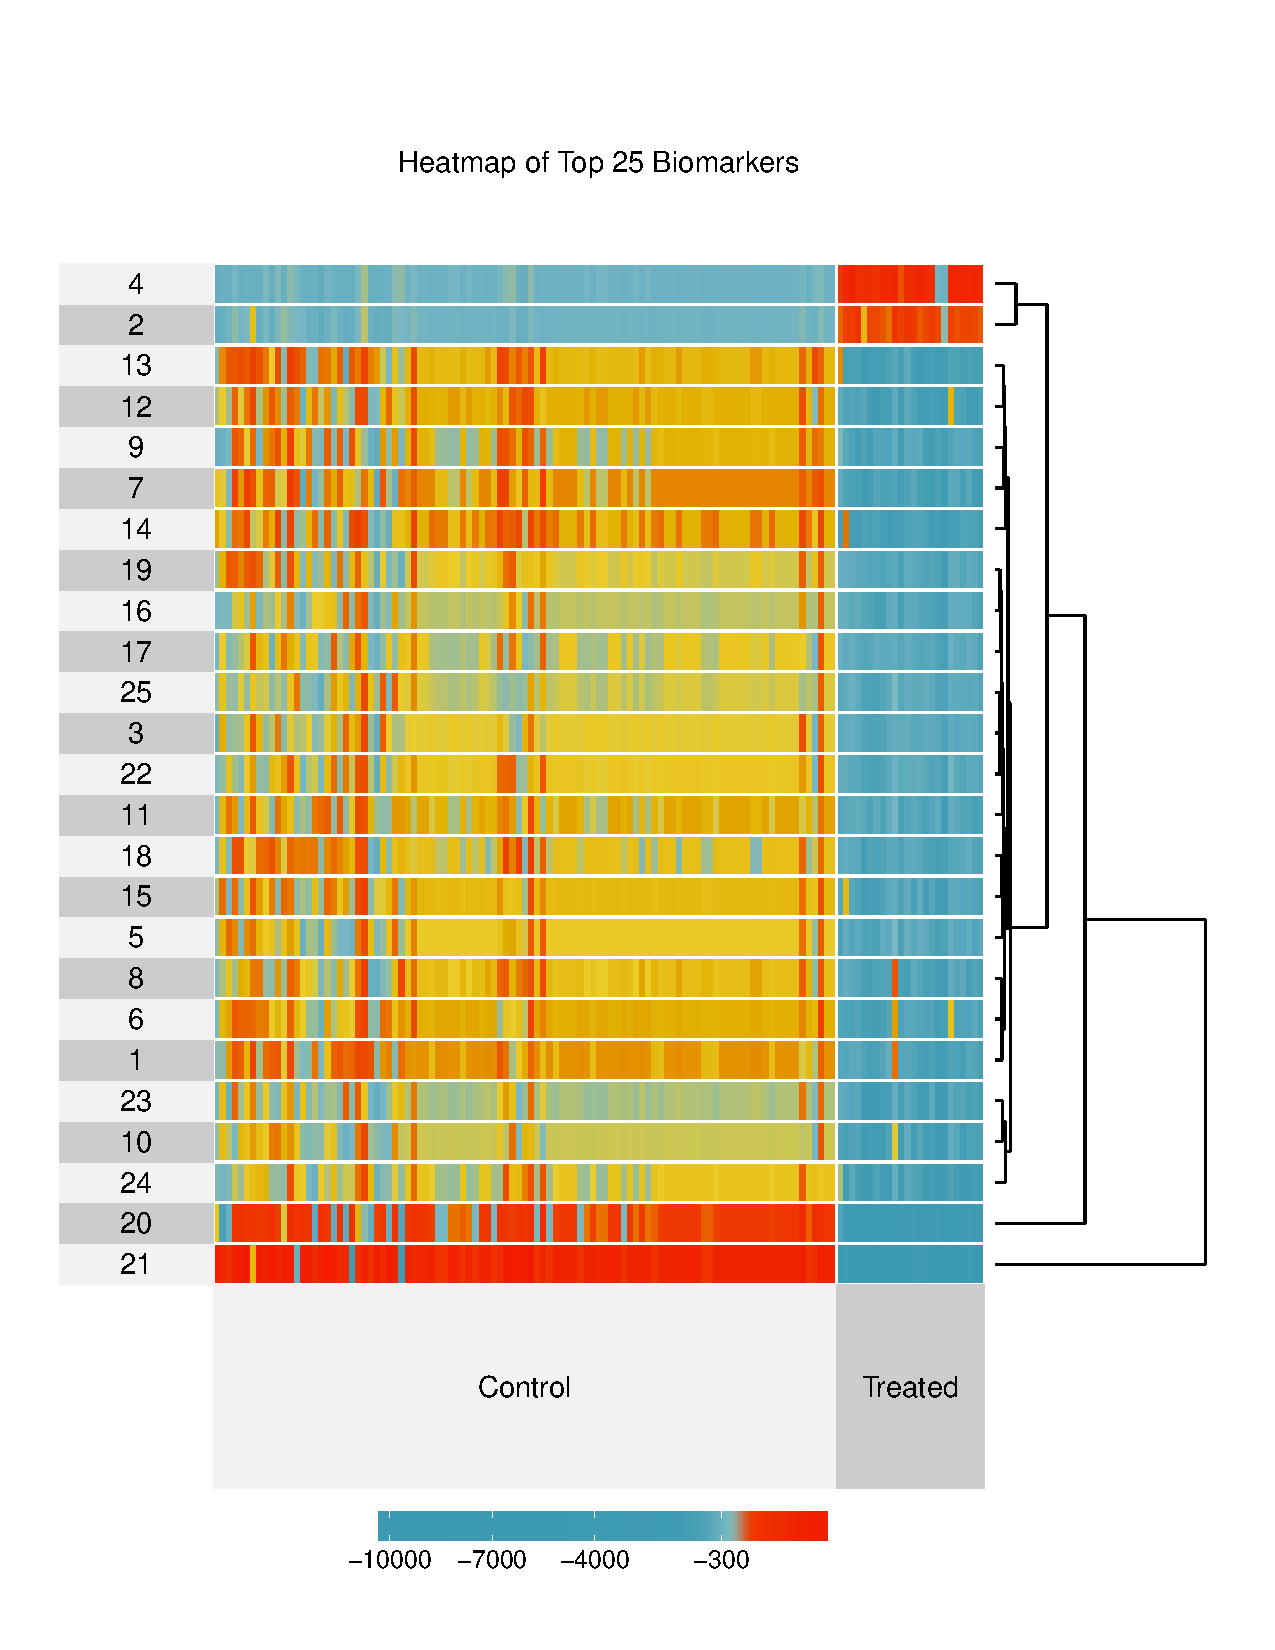
\includegraphics[scale=0.75]{figs/superheatmap.pdf}
  \caption{Heatmap of the ATE estimates. Blue indicates a depression in the
    ATE, while red indicates an increase in the ATE, based on exposure to the
    maximal level of benzene as opposed to the minimal level.}
\end{figure}

As expected, Limma reduced the spread of the standard deviation estimates of
the influence curve by probe ($\widetilde{\sigma}^b_n$) across the $\sim 20,000$
probes, and the corresponding Wald statistics for testing the target parameter,
in comparison of using the original standard error, $\sigma^b_n$. The results of
our analysis indicate that the moderated t-statistic applied to the ATE
constitutes a powerful approach for assessing variable importance, based on
exposure, in the context of high-dimensional investigations of biomarkers. We
conclude that using this adaptation of TMLE, complimented by the moderated
t-statistic of the R package LIMMA, reduces the variability of standard errors
and reduces the number of significant probes, leading to more stable and robust
inference, while providing the opportunity to evaluate biomarkers in the context
of statistical parameters of scientific relevance, such as the average treatment
effect focused on in the above example.


\printbibliography

% \appendix
% \chapter{More Monticello Candidates}

\end{document}
